\documentclass[12pt]{beamer}

\usepackage[utf8]{inputenc}
\usepackage[T2A]{fontenc}
\usepackage[english,russian]{babel}

\usepackage{pscyr}          % Cyrillic fonts

% Стиль презентации
\usetheme{Szeged}
%\usefonttheme[]{serif}
\usefonttheme{professionalfonts}

%\setbeamerfont{structure}{family=\rmfamily}
\usecolortheme{lily}

\begin{document}

\title{Анализ безопасности протокола WEP в компьютерных сетях стандарта 802.11 WLAN}
\author{Фролов В.В.}
\date{}

% Создание заглавной страницы
\frame{\titlepage} 
% Автоматическая генерация содержания


\begin{frame}{Задачи}

\begin{itemize}
    \item изучить протокол WEP, процесс обмена пакетами и обеспечение аутентификации и конфиденциальности в сетях стандарта 802.11 WLAN
    \item исследовать возможные атаки и реализовать атаку с фрагментацией на WEP
    \item провести анализ безопасности WEP
    \item рассмотреть условия работы труда на рабочем месте и расчитать КЕО для города Харькова
\end{itemize}

\end{frame} 


\begin{frame}{Передача пакетов в сетях стандарта 802.11 WLAN}

\begin{figure}
    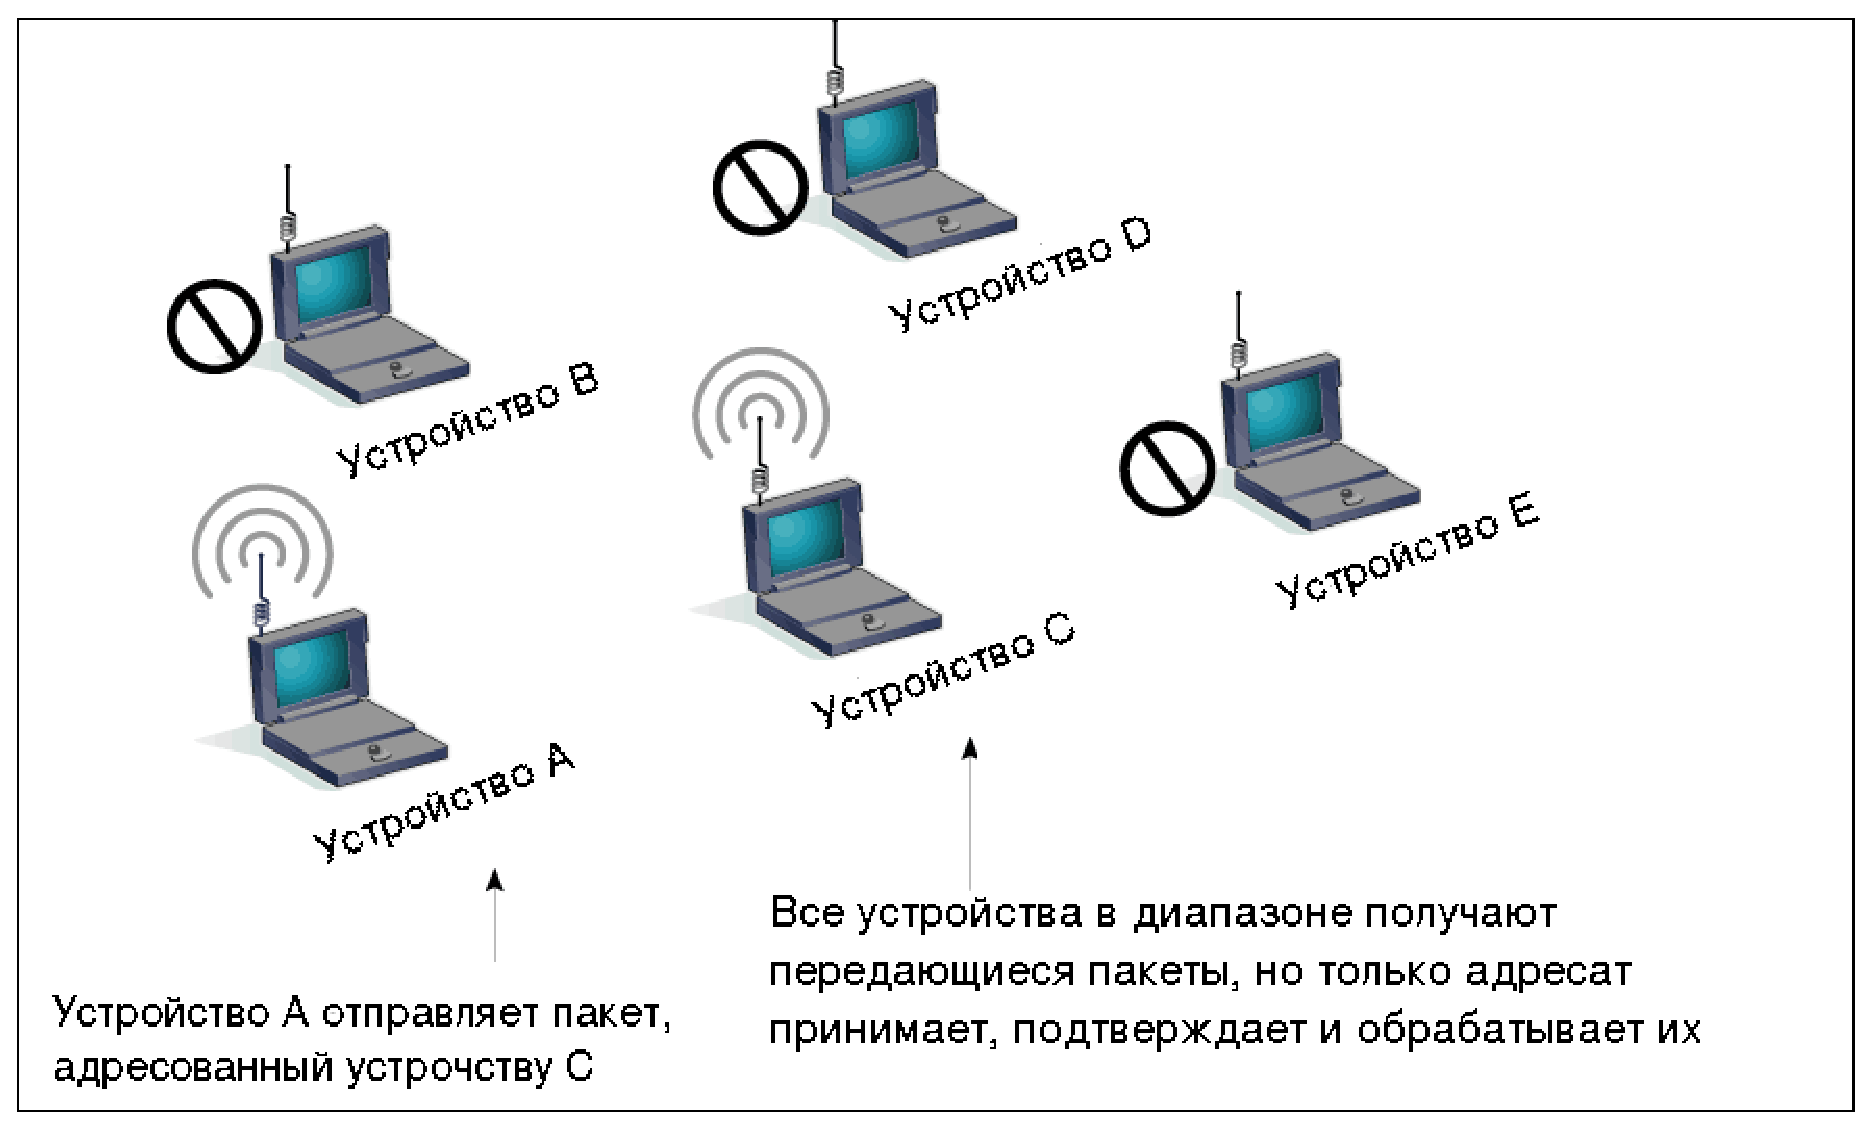
\includegraphics[width=9cm]{graphics/wlan_diagram.eps}
\end{figure}

\end{frame} 


\begin{frame}{Классификация атак на протокол WEP}

\begin{figure}
    \includegraphics[width=10cm]{graphics/wep_attacks_classification.eps}
\end{figure}

%\begin{itemize}
%    \item
%\end{itemize}

\end{frame} 


\begin{frame}{Алгоритм атаки с фрагментацией}

\begin{figure}
    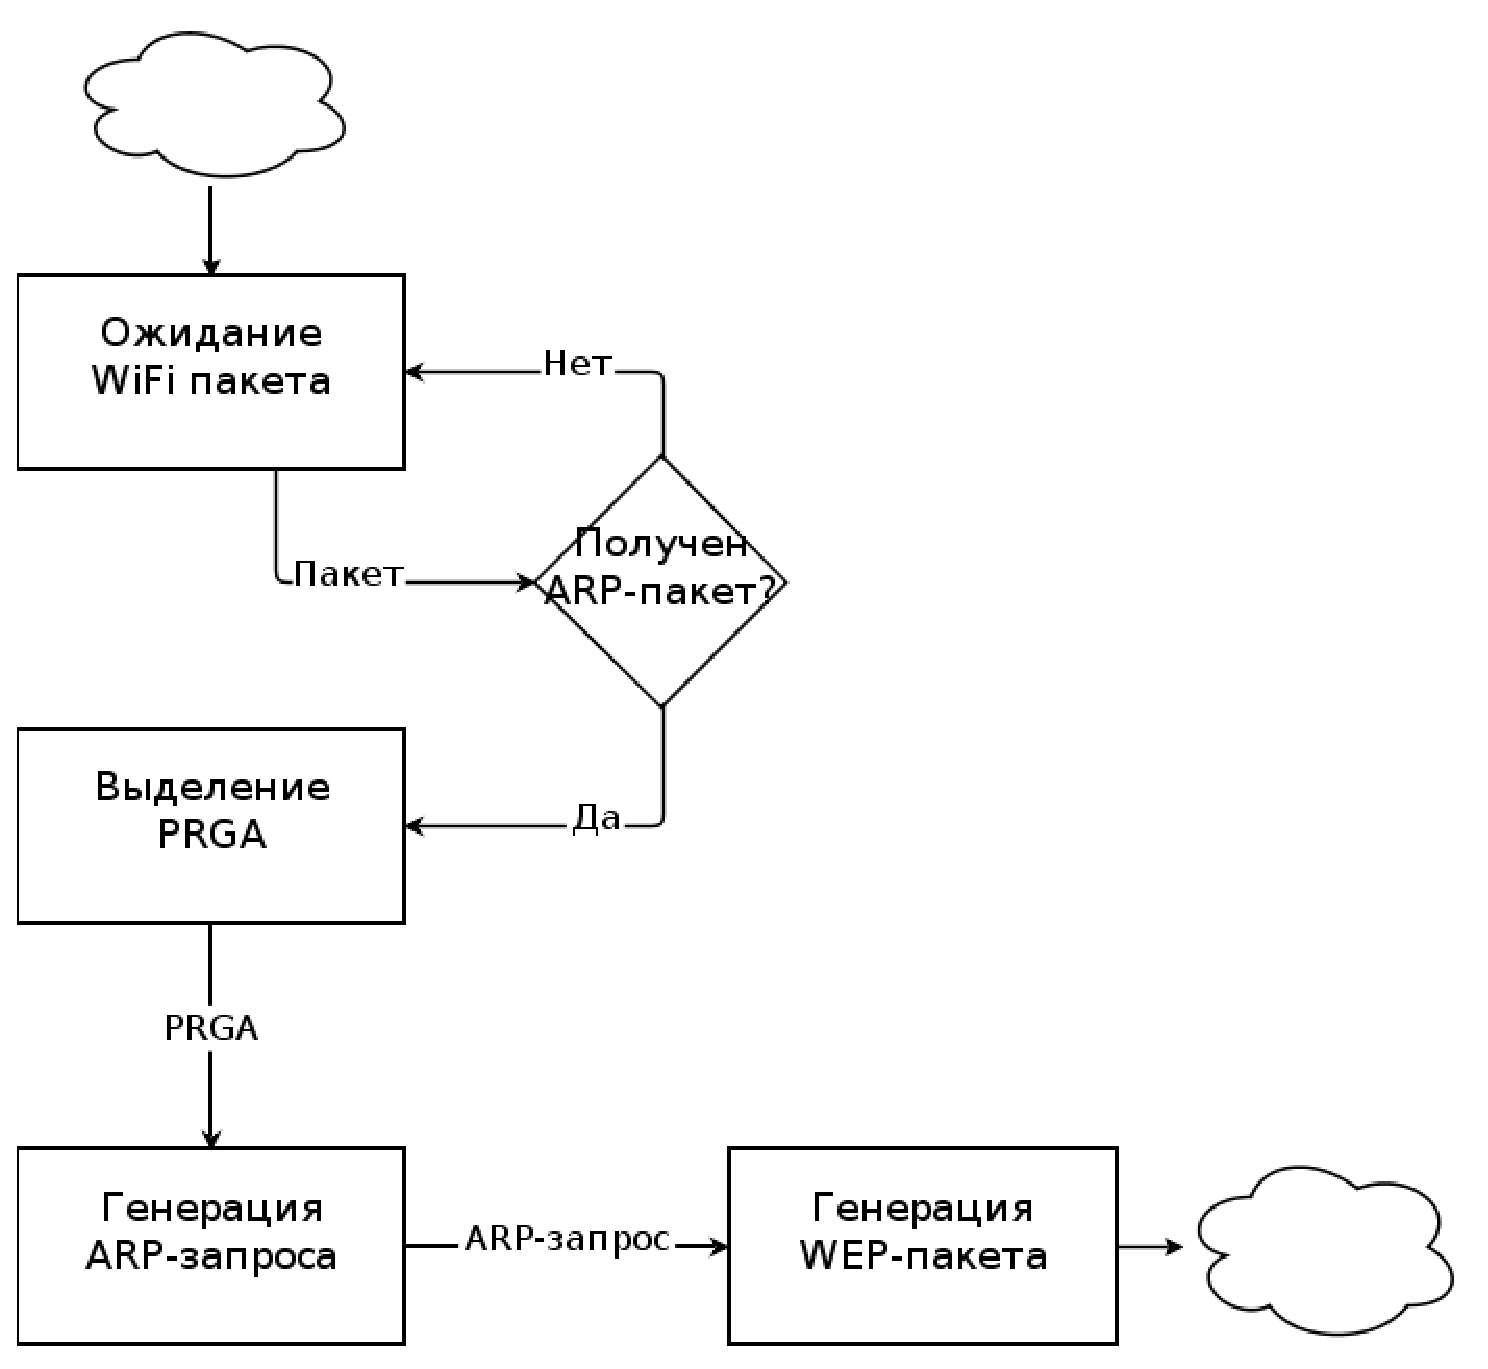
\includegraphics[width=7cm]{graphics/fragment_program_algo.eps}
\end{figure}

\end{frame} 


\begin{frame}{Атака с фрагментацией}

\begin{figure}
    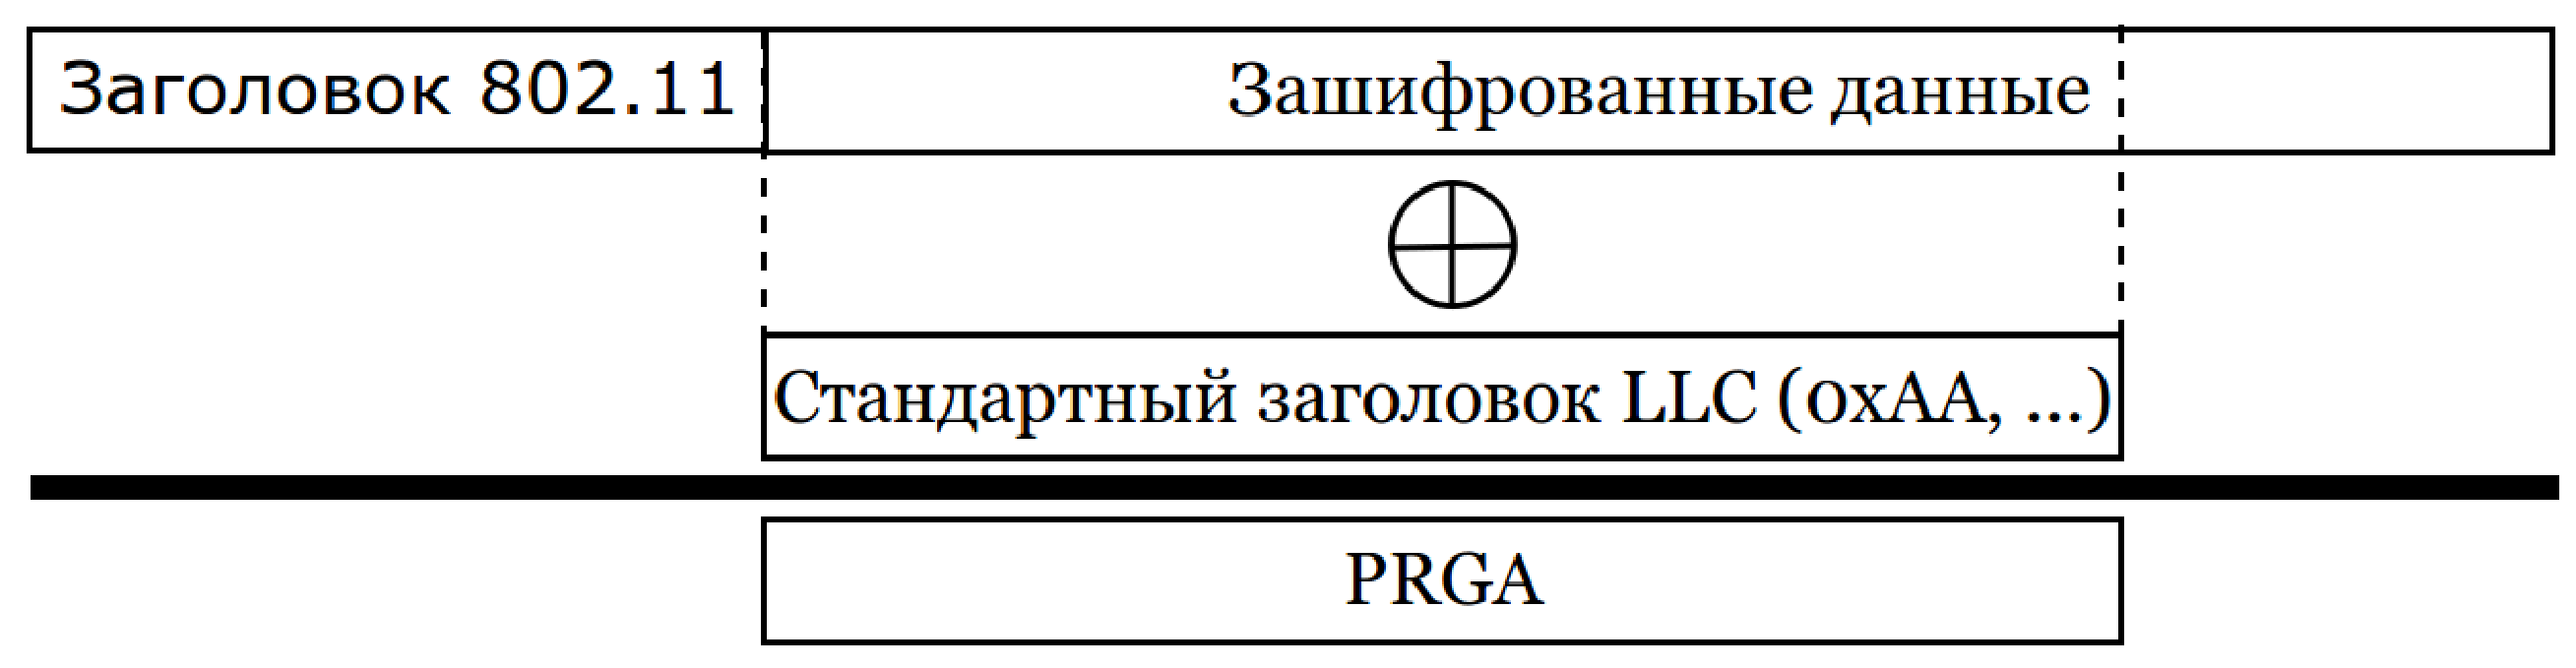
\includegraphics[width=10cm]{graphics/restore_part_of_gamma.eps}
\end{figure}

\begin{figure}
    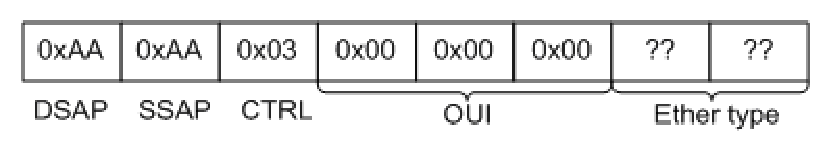
\includegraphics[width=10cm]{graphics/default_llc_header.eps}
\end{figure}

\end{frame} 


\begin{frame}{}

\begin{itemize}
    \item
\end{itemize}

\end{frame} 


\begin{frame}{Охрана труда}

\begin{itemize}
    \item Коеффициент ествественного освещения равен 1.8\%
\end{itemize}

\end{frame} 


\begin{frame}{Выводы}

\begin{itemize}
    \item Исследован процесс обмена пакетами и обеспечение безопасности в сетях стандарта 802.11 WLAN
    \item Рассмотрены возможные атаки на протокол WEP
    \item Реализована атака с фрагментацией
    \item Проведён анализ безопасности WEP
    \item Расчитан коеффициент естественного освещения для города Харькова
\end{itemize}

\end{frame} 


\begin{frame}{}

\begin{center}
    Спасибо за внимание.
\end{center}

\end{frame}

\end{document}
